\section{Background and Motivation}
\label{sec:background}

\subsection{Average versus marginal carbon intensity}
The carbon intensity of grid-supplied electricity is not a single number. The \emph{average} intensity records the emissions of the average electron delivered to a balancing area over a window, obtained by dividing total emissions by total demand. The \emph{marginal} intensity records the emissions of the next electron: it is the intensity of the marginal generator that ramps up or down to absorb an incremental change in demand. Because the marginal generator is typically fossil and the average mix contains zero-carbon baseload, the two signals differ, often by a factor of two or three, and they are poorly correlated in the hours that matter for scheduling decisions~\cite{sukprasert2024implications}. A workload that reduces demand in an hour of low average intensity but high marginal intensity has a small effect on emissions, because the curtailed generation is clean baseload that would have been used anyway; the same reduction in an hour of high marginal intensity displaces fossil generation and yields a large saving. Sukprasert et al.\ show that using the average signal in place of the marginal one systematically misranks candidate deferral windows and can yield carbon-aware optimisations that increase emissions~\cite{sukprasert2024implications}. The Green Mirage result extends this to the method of estimation: location- and market-based accounting methods disagree, and the optimisation efficacy of a carbon-aware policy depends sharply on which method the signal uses~\cite{maji2024green}. Figure~\ref{fig:marginal-vs-avg} illustrates the divergence on a representative day: the marginal signal swings sharply between fossil-ramp peaks and renewable-surplus troughs, while the average signal lags and compresses both, so the two signals recommend different deferral targets.

\begin{figure}[tb]
\centering
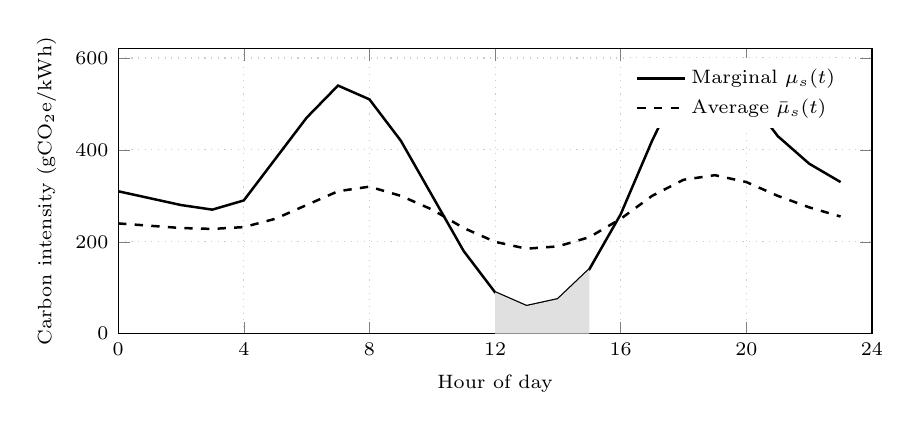
\begin{tikzpicture}
\begin{axis}[
  width=0.92\columnwidth, height=5.2cm,
  xlabel={Hour of day}, ylabel={Carbon intensity (gCO\textsubscript{2}e/kWh)},
  xmin=0, xmax=24, ymin=0, ymax=620,
  xtick={0,4,8,12,16,20,24},
  legend pos=north east, legend style={font=\scriptsize, draw=none},
  legend cell align=left,
  grid=both, grid style={dotted, black!20},
  tick label style={font=\scriptsize}, label style={font=\scriptsize},
  every axis plot/.append style={line width=0.9pt}
]
% Marginal intensity: sharp peaks at fossil ramp hours, deep troughs at solar surplus
\addplot[black, mark=none] coordinates {
 (0,310)(1,295)(2,280)(3,270)(4,290)(5,380)(6,470)(7,540)(8,510)
 (9,420)(10,300)(11,180)(12,90)(13,60)(14,75)(15,140)(16,260)
 (17,420)(18,560)(19,590)(20,520)(21,430)(22,370)(23,330)
};
% Average intensity: smoother, lags marginal, never as deep or as high
\addplot[black, dashed, mark=none] coordinates {
 (0,240)(1,235)(2,230)(3,228)(4,232)(5,250)(6,280)(7,310)(8,320)
 (9,300)(10,270)(11,230)(12,200)(13,185)(14,190)(15,210)(16,250)
 (17,300)(18,335)(19,345)(20,330)(21,300)(22,275)(23,255)
};
% Shaded surplus window 12:00-15:00
\addplot[fill=black!12, draw=none] coordinates {
 (12,0)(12,90)(13,60)(14,75)(15,140)(15,0)
} \closedcycle;
\legend{Marginal $\mu_s(t)$, Average $\bar\mu_s(t)$}
\end{axis}
\end{tikzpicture}
\caption{Marginal versus average carbon intensity over a representative
day (mock trace, calibrated to the divergence reported in
prior measurement work). The shaded band marks a renewable-surplus
window where marginal intensity drops well below the average. A
scheduler on the average signal defers into hours 10--12, where the
average is low but the marginal generator is still fossil; a scheduler
on the marginal signal defers into the shaded window, where the
incremental electron is genuinely clean. The gap between the two curves
is the carbon saving \textsc{CarbonShift} recovers.}
\label{fig:marginal-vs-avg}
\end{figure}


The sunk-carbon critique~\cite{bashir2024sunk} attacks the operational-only view from a second direction. Hardware has already absorbed embodied carbon at manufacture, and the relevant question for a scheduling decision is the marginal carbon of the decision itself, not the cumulative footprint of the hardware. A scheduler that counts only operational energy and ignores the embodied cost can, paradoxically, defer a job into a clean hour that triggers a cold start, where the amortised embodied carbon of the new container exceeds the operational carbon saved. Combining the marginal signal with an embodied-amortisation term is, to our knowledge, unaddressed in the carbon-aware serverless literature.

\subsection{Carbon-aware workload shifting}
The carbon-aware shifting literature has matured rapidly. Asadov et al.\ review the field and propose a spatio-temporal shifting algorithm, but the formulation places an average intensity in the objective and treats the site set as static~\cite{asadov2025carbonaware}. Patel et al.\ argue for an agile pathway to carbon-aware clouds built on the marginal signal in principle but stop short of a scheduler that consumes it online~\cite{patel2024agile}. Radhakrishnan uses deep reinforcement learning to place Kubernetes workloads on a marginal signal but treats the workload set as coarse-grained batch jobs rather than per-invocation FaaS~\cite{radhakrishnan2024carbonaware}. Caribou shifts serverless applications geospatially between regions using marginal intensity, but the shift is spatial only and does not model the temporal deferral of a single job across a renewable-surplus window~\cite{gsteiger2024caribou}. Rodrigues et al.\ apply temporal deferral to inter-datacentre data transfers~\cite{rodrigues2025carbonaware}. Ozkan and Ozkan present a federated carbon-intelligence framework for AI workloads~\cite{ozkan2025federated}, and Shingne designs an iterative predictive carbon-aware scheduler for cloud--fog--edge~\cite{shingne2025design}; both emphasise the predictive element but neither gives an online guarantee against an offline optimum that knows the marginal trajectory.

The continuum background motivates the placement of the problem. Cloud--edge continuum modelling work~\cite{patel2024modeling,aldulaimy2024computing} formalises the computing continuum and its heterogeneity, and service-placement work on the continuum~\cite{rac2024costaware,soumplis2024performance,bellavista2024exploiting} formalises the cost of being in the wrong tier. None of these threads couples the marginal carbon signal to the per-invocation deferral decision, which is the gap this paper targets.

\subsection{Serverless cold starts and scheduling}
Cold starts are the defining operational cost of FaaS. When an invocation arrives for a function with no warm instance, a container must be created, initialised, and code loaded; the latency penalty this imposes on the user is the cold-start cost, and the carbon cost is the extra energy and the amortised embodied carbon of the new container. Mitigation work splits broadly between caching and prediction. RainbowCake caches layers~\cite{yu2024rainbowcake}; CodeCrunch predicts invocations and warmups up selectively, with an explicit cost model on the warmup~\cite{roy2024codecrunch}; vertical scaling handles bursts~\cite{calavaro2025beyond}; cross-edge caching places functions probabilistically across edges~\cite{chen2024crossedge}; deep reinforcement learning orchestrates FaaS across the continuum~\cite{khansari2024deep}. Chen et al.\ survey cold-start latency optimisation strategies~\cite{chen2026cold}; Hong et al.\ study the interplay of autoscaling and QoS~\cite{hong2024analysis}. None of these threads charges the cold-start decision with a carbon cost; the warmup that mitigates latency also amortises embodied carbon, and the decision to warm versus defer is the same decision seen from two angles. Bringing the marginal carbon signal into this decision is the second gap the paper targets.

\subsection{The gap}
Three observations follow from the background. First, the marginal carbon signal is known to be the correct one but is seldom consumed online by per-invocation schedulers, and never with a competitive-ratio guarantee. Second, renewable surpluses arrive as short windows that are predictable only hours ahead, so the optimisation horizon must be short and the guarantee must hold under forecast error. Third, the cold-start decision and the deferral decision interact through embodied carbon: a deferral that triggers a cold start can be net-negative. No prior scheme addresses all three together. Sections~\ref{sec:model} and~\ref{sec:algorithm} build a model and an algorithm that do.
